\documentclass[man, fleqn, noextraspace,floatsintext]{apa6}
\usepackage{lmodern}
\usepackage{amssymb,amsmath}
\usepackage{ifxetex,ifluatex}
\usepackage{fixltx2e} % provides \textsubscript
\ifnum 0\ifxetex 1\fi\ifluatex 1\fi=0 % if pdftex
  \usepackage[T1]{fontenc}
  \usepackage[utf8]{inputenc}
\else % if luatex or xelatex
  \ifxetex
    \usepackage{mathspec}
  \else
    \usepackage{fontspec}
  \fi
  \defaultfontfeatures{Ligatures=TeX,Scale=MatchLowercase}
\fi
% use upquote if available, for straight quotes in verbatim environments
\IfFileExists{upquote.sty}{\usepackage{upquote}}{}
% use microtype if available
\IfFileExists{microtype.sty}{%
\usepackage{microtype}
\UseMicrotypeSet[protrusion]{basicmath} % disable protrusion for tt fonts
}{}
\usepackage{hyperref}
\hypersetup{unicode=true,
            pdftitle={EDLD 610 Final Project},
            pdfauthor={Woocheol Kim~\& Jessica Canfield},
            pdfkeywords={sports, NBA, NHL, NFL, MLB, NCAAF},
            pdfborder={0 0 0},
            breaklinks=true}
\urlstyle{same}  % don't use monospace font for urls
\usepackage{color}
\usepackage{fancyvrb}
\newcommand{\VerbBar}{|}
\newcommand{\VERB}{\Verb[commandchars=\\\{\}]}
\DefineVerbatimEnvironment{Highlighting}{Verbatim}{commandchars=\\\{\}}
% Add ',fontsize=\small' for more characters per line
\usepackage{framed}
\definecolor{shadecolor}{RGB}{248,248,248}
\newenvironment{Shaded}{\begin{snugshade}}{\end{snugshade}}
\newcommand{\AlertTok}[1]{\textcolor[rgb]{0.94,0.16,0.16}{#1}}
\newcommand{\AnnotationTok}[1]{\textcolor[rgb]{0.56,0.35,0.01}{\textbf{\textit{#1}}}}
\newcommand{\AttributeTok}[1]{\textcolor[rgb]{0.77,0.63,0.00}{#1}}
\newcommand{\BaseNTok}[1]{\textcolor[rgb]{0.00,0.00,0.81}{#1}}
\newcommand{\BuiltInTok}[1]{#1}
\newcommand{\CharTok}[1]{\textcolor[rgb]{0.31,0.60,0.02}{#1}}
\newcommand{\CommentTok}[1]{\textcolor[rgb]{0.56,0.35,0.01}{\textit{#1}}}
\newcommand{\CommentVarTok}[1]{\textcolor[rgb]{0.56,0.35,0.01}{\textbf{\textit{#1}}}}
\newcommand{\ConstantTok}[1]{\textcolor[rgb]{0.00,0.00,0.00}{#1}}
\newcommand{\ControlFlowTok}[1]{\textcolor[rgb]{0.13,0.29,0.53}{\textbf{#1}}}
\newcommand{\DataTypeTok}[1]{\textcolor[rgb]{0.13,0.29,0.53}{#1}}
\newcommand{\DecValTok}[1]{\textcolor[rgb]{0.00,0.00,0.81}{#1}}
\newcommand{\DocumentationTok}[1]{\textcolor[rgb]{0.56,0.35,0.01}{\textbf{\textit{#1}}}}
\newcommand{\ErrorTok}[1]{\textcolor[rgb]{0.64,0.00,0.00}{\textbf{#1}}}
\newcommand{\ExtensionTok}[1]{#1}
\newcommand{\FloatTok}[1]{\textcolor[rgb]{0.00,0.00,0.81}{#1}}
\newcommand{\FunctionTok}[1]{\textcolor[rgb]{0.00,0.00,0.00}{#1}}
\newcommand{\ImportTok}[1]{#1}
\newcommand{\InformationTok}[1]{\textcolor[rgb]{0.56,0.35,0.01}{\textbf{\textit{#1}}}}
\newcommand{\KeywordTok}[1]{\textcolor[rgb]{0.13,0.29,0.53}{\textbf{#1}}}
\newcommand{\NormalTok}[1]{#1}
\newcommand{\OperatorTok}[1]{\textcolor[rgb]{0.81,0.36,0.00}{\textbf{#1}}}
\newcommand{\OtherTok}[1]{\textcolor[rgb]{0.56,0.35,0.01}{#1}}
\newcommand{\PreprocessorTok}[1]{\textcolor[rgb]{0.56,0.35,0.01}{\textit{#1}}}
\newcommand{\RegionMarkerTok}[1]{#1}
\newcommand{\SpecialCharTok}[1]{\textcolor[rgb]{0.00,0.00,0.00}{#1}}
\newcommand{\SpecialStringTok}[1]{\textcolor[rgb]{0.31,0.60,0.02}{#1}}
\newcommand{\StringTok}[1]{\textcolor[rgb]{0.31,0.60,0.02}{#1}}
\newcommand{\VariableTok}[1]{\textcolor[rgb]{0.00,0.00,0.00}{#1}}
\newcommand{\VerbatimStringTok}[1]{\textcolor[rgb]{0.31,0.60,0.02}{#1}}
\newcommand{\WarningTok}[1]{\textcolor[rgb]{0.56,0.35,0.01}{\textbf{\textit{#1}}}}
\usepackage{graphicx,grffile}
\makeatletter
\def\maxwidth{\ifdim\Gin@nat@width>\linewidth\linewidth\else\Gin@nat@width\fi}
\def\maxheight{\ifdim\Gin@nat@height>\textheight\textheight\else\Gin@nat@height\fi}
\makeatother
% Scale images if necessary, so that they will not overflow the page
% margins by default, and it is still possible to overwrite the defaults
% using explicit options in \includegraphics[width, height, ...]{}
\setkeys{Gin}{width=\maxwidth,height=\maxheight,keepaspectratio}
\IfFileExists{parskip.sty}{%
\usepackage{parskip}
}{% else
\setlength{\parindent}{0pt}
\setlength{\parskip}{6pt plus 2pt minus 1pt}
}
\setlength{\emergencystretch}{3em}  % prevent overfull lines
\providecommand{\tightlist}{%
  \setlength{\itemsep}{0pt}\setlength{\parskip}{0pt}}
\setcounter{secnumdepth}{0}
% Redefines (sub)paragraphs to behave more like sections
\ifx\paragraph\undefined\else
\let\oldparagraph\paragraph
\renewcommand{\paragraph}[1]{\oldparagraph{#1}\mbox{}}
\fi
\ifx\subparagraph\undefined\else
\let\oldsubparagraph\subparagraph
\renewcommand{\subparagraph}[1]{\oldsubparagraph{#1}\mbox{}}
\fi

%%% Use protect on footnotes to avoid problems with footnotes in titles
\let\rmarkdownfootnote\footnote%
\def\footnote{\protect\rmarkdownfootnote}


  \title{EDLD 610 Final Project}
    \author{Woocheol Kim\textsuperscript{1}~\& Jessica Canfield\textsuperscript{1}}
    \date{}
  
\shorttitle{Exploring Trends in Major League Sports }
\affiliation{
\vspace{0.5cm}
\textsuperscript{1} University of Oregon}
\keywords{sports, NBA, NHL, NFL, MLB, NCAAF}
\usepackage{csquotes}
\usepackage{upgreek}
\captionsetup{font=singlespacing,justification=justified}

\usepackage{longtable}
\usepackage{lscape}
\usepackage{multirow}
\usepackage{tabularx}
\usepackage[flushleft]{threeparttable}
\usepackage{threeparttablex}

\newenvironment{lltable}{\begin{landscape}\begin{center}\begin{ThreePartTable}}{\end{ThreePartTable}\end{center}\end{landscape}}

\makeatletter
\newcommand\LastLTentrywidth{1em}
\newlength\longtablewidth
\setlength{\longtablewidth}{1in}
\newcommand{\getlongtablewidth}{\begingroup \ifcsname LT@\roman{LT@tables}\endcsname \global\longtablewidth=0pt \renewcommand{\LT@entry}[2]{\global\advance\longtablewidth by ##2\relax\gdef\LastLTentrywidth{##2}}\@nameuse{LT@\roman{LT@tables}} \fi \endgroup}


\usepackage{lineno}

\linenumbers

\authornote{Jessica Canfield \& Woocheol Kim are both Marketing PhD students at the University of Oregon.

Correspondence concerning this article should be addressed to Woocheol Kim, 1208 University St, Eugene, OR 97403. E-mail: \href{mailto:wkim4@uoregon.edu}{\nolinkurl{wkim4@uoregon.edu}}}

\abstract{
Marketing research has frequently used the context of sports to explore one facet of consumption. Additionally, the data within the sports realm is well-documented and detailed across time which allows for analyses to be tracked across time and different locations. While the current analysis is mainly exploratory in nature the goal of this project is to familiarize ourselves with this dataset prior to using it in future marketing studies. In this project specifically we look at how the 2008 financial crisis impacts ticket price for professional sports teams. However, in the future we plan to use this data in conjunction with other datasets that have unique time and location identifiers to look more specifically at how consumers engage with sports in reaction to other events occuring simultaneously, whether that be financial crises, political uncertainty, or natural disasters.


}

\begin{document}
\maketitle

\hypertarget{introduction-and-overview}{%
\section{Introduction and Overview}\label{introduction-and-overview}}

Humphreys (2010) explores the impact of the global financial crisis on sport in North America. He finds that while attendance and franchise values declined slightly, and a few teams experienced financial problems, the nature of the sport product and institutional factors associated with the sports industry have, so far, insulted professional sport from significant negative impacts. Coates and Humphreys (2007) investigate the demand for attendance at professional sporting events using a data set that includes ticket prices and a price index reflecting prices for ancillary goods associated with attendance. Both mathematical modeling and empirical methodology are used in their research. (see Coates \& Humphreys, 2007).

\begin{Shaded}
\begin{Highlighting}[]
\NormalTok{mlb <-}\StringTok{ }\KeywordTok{import}\NormalTok{(}\KeywordTok{here}\NormalTok{(}\StringTok{"Data"}\NormalTok{, }\StringTok{"MLB.xlsx"}\NormalTok{)) }\OperatorTok
\StringTok{  }\KeywordTok{characterize}\NormalTok{() }\OperatorTok
\StringTok{  }\KeywordTok{clean_names}\NormalTok{() }\OperatorTok\StringTok{ }
\StringTok{  }\KeywordTok{select}\NormalTok{(sport, team, year, capacity, }
\NormalTok{         attend_tot, attend_avg, games, }
\NormalTok{         ticket_price, home_wins) }\OperatorTok\StringTok{ }
\StringTok{  }\KeywordTok{as_tibble}\NormalTok{()}

\NormalTok{mlb <-}\StringTok{ }\NormalTok{mlb }\OperatorTok\StringTok{ }
\StringTok{  }\KeywordTok{mutate}\NormalTok{(}\DataTypeTok{capacity =} \KeywordTok{as.numeric}\NormalTok{(capacity), }
         \DataTypeTok{attend_tot =} \KeywordTok{as.numeric}\NormalTok{(attend_tot),  }
         \DataTypeTok{attend_avg =} \KeywordTok{as.numeric}\NormalTok{(attend_avg),}
         \DataTypeTok{games =} \KeywordTok{as.numeric}\NormalTok{(games), }
         \DataTypeTok{ticket_price =} \KeywordTok{as.numeric}\NormalTok{(ticket_price), }
         \DataTypeTok{home_wins =} \KeywordTok{as.numeric}\NormalTok{(home_wins))}

\CommentTok{#is.character(mlb$capacity)}
\end{Highlighting}
\end{Shaded}

\begin{Shaded}
\begin{Highlighting}[]
\NormalTok{nba <-}\StringTok{ }\KeywordTok{import}\NormalTok{(}\KeywordTok{here}\NormalTok{(}\StringTok{"Data"}\NormalTok{, }\StringTok{"NBA.xlsx"}\NormalTok{)) }\OperatorTok
\StringTok{  }\KeywordTok{characterize}\NormalTok{() }\OperatorTok\StringTok{  }
\StringTok{  }\KeywordTok{clean_names}\NormalTok{()}\OperatorTok\StringTok{ }
\StringTok{  }\KeywordTok{select}\NormalTok{(sport, team, year, capacity, }
\NormalTok{         attend_tot, attend_avg, games, }
\NormalTok{         ticket_price, home_win) }\OperatorTok\StringTok{ }
\StringTok{  }\KeywordTok{as_tibble}\NormalTok{() }\OperatorTok\StringTok{ }
\StringTok{  }\KeywordTok{rename}\NormalTok{(}\DataTypeTok{home_wins =}\NormalTok{ home_win) }\OperatorTok\StringTok{ }
\StringTok{  }\KeywordTok{as_tibble}\NormalTok{()}

\NormalTok{nba <-}\StringTok{ }\NormalTok{nba }\OperatorTok\StringTok{ }\KeywordTok{mutate}\NormalTok{(}\DataTypeTok{capacity =} \KeywordTok{as.numeric}\NormalTok{(capacity), }
                      \DataTypeTok{attend_tot =} \KeywordTok{as.numeric}\NormalTok{(attend_tot), }
                      \DataTypeTok{attend_avg =} \KeywordTok{as.numeric}\NormalTok{(attend_avg), }
                      \DataTypeTok{games =} \KeywordTok{as.numeric}\NormalTok{(games), }
                      \DataTypeTok{ticket_price =} \KeywordTok{as.numeric}\NormalTok{(ticket_price), }
                      \DataTypeTok{home_wins =} \KeywordTok{as.numeric}\NormalTok{(home_wins))}

\NormalTok{ncaaf <-}\StringTok{ }\KeywordTok{import}\NormalTok{(}\KeywordTok{here}\NormalTok{(}\StringTok{"Data"}\NormalTok{, }\StringTok{"NCAAF.xlsx"}\NormalTok{)) }\OperatorTok
\StringTok{  }\KeywordTok{characterize}\NormalTok{() }\OperatorTok\StringTok{  }
\StringTok{  }\KeywordTok{clean_names}\NormalTok{() }\OperatorTok\StringTok{ }
\StringTok{  }\KeywordTok{select}\NormalTok{(sport, team, year, capacity,}
\NormalTok{         attend_tot, attend_avg, games, }
\NormalTok{         ticket_price, home_wins) }\OperatorTok\StringTok{ }
\StringTok{  }\KeywordTok{as_tibble}\NormalTok{()}

\NormalTok{nfl <-}\StringTok{ }\KeywordTok{import}\NormalTok{(}\KeywordTok{here}\NormalTok{(}\StringTok{"Data"}\NormalTok{, }\StringTok{"NFL.xlsx"}\NormalTok{)) }\OperatorTok
\StringTok{  }\KeywordTok{characterize}\NormalTok{() }\OperatorTok\StringTok{  }
\StringTok{  }\KeywordTok{clean_names}\NormalTok{()}\OperatorTok\StringTok{ }
\StringTok{  }\KeywordTok{select}\NormalTok{(sport, team, year, capacity, }
\NormalTok{         attend_tot, attend_avg, games, }
\NormalTok{         ticket_price, home_wins) }\OperatorTok\StringTok{ }
\StringTok{  }\KeywordTok{as_tibble}\NormalTok{()}

\NormalTok{nfl <-}\StringTok{ }\NormalTok{nfl }\OperatorTok\StringTok{ }\KeywordTok{mutate}\NormalTok{(}\DataTypeTok{attend_tot =} \KeywordTok{as.numeric}\NormalTok{(attend_tot),  }
                      \DataTypeTok{attend_avg =} \KeywordTok{as.numeric}\NormalTok{(attend_avg),}
                      \DataTypeTok{games =} \KeywordTok{as.numeric}\NormalTok{(games), }
                      \DataTypeTok{ticket_price =} \KeywordTok{as.numeric}\NormalTok{(ticket_price), }
                      \DataTypeTok{home_wins =} \KeywordTok{as.numeric}\NormalTok{(home_wins))}

\NormalTok{nhl <-}\StringTok{ }\KeywordTok{import}\NormalTok{(}\KeywordTok{here}\NormalTok{(}\StringTok{"Data"}\NormalTok{, }\StringTok{"NHL.xlsx"}\NormalTok{)) }\OperatorTok
\StringTok{  }\KeywordTok{characterize}\NormalTok{() }\OperatorTok\StringTok{  }
\StringTok{  }\KeywordTok{clean_names}\NormalTok{()}\OperatorTok\StringTok{ }
\StringTok{  }\KeywordTok{select}\NormalTok{(sport, team, year, capacity, }
\NormalTok{         attend_tot, attend_avg, games, }
\NormalTok{         ticket_price, home_wins) }\OperatorTok\StringTok{ }
\StringTok{  }\KeywordTok{as_tibble}\NormalTok{() }

\NormalTok{nhl <-}\StringTok{ }\NormalTok{nhl }\OperatorTok\StringTok{ }\KeywordTok{mutate}\NormalTok{(}\DataTypeTok{attend_tot =} \KeywordTok{as.numeric}\NormalTok{(attend_tot),}
                      \DataTypeTok{attend_avg =} \KeywordTok{as.numeric}\NormalTok{(attend_avg), }
                      \DataTypeTok{games =} \KeywordTok{as.numeric}\NormalTok{(games), }
                      \DataTypeTok{ticket_price =} \KeywordTok{as.numeric}\NormalTok{(ticket_price),}
                      \DataTypeTok{home_wins =} \KeywordTok{as.numeric}\NormalTok{(home_wins))}

\NormalTok{sports <-}\StringTok{ }\KeywordTok{bind_rows}\NormalTok{(mlb, nba, ncaaf, nfl, nhl)}\OperatorTok\StringTok{ }
\StringTok{  }\KeywordTok{as_tibble}\NormalTok{()}
\end{Highlighting}
\end{Shaded}

\begin{Shaded}
\begin{Highlighting}[]
\NormalTok{sports <-}\StringTok{ }\NormalTok{sports }\OperatorTok
\StringTok{  }\KeywordTok{mutate}\NormalTok{(}\DataTypeTok{home_wins_pct =}\NormalTok{ home_wins}\OperatorTok{/}\NormalTok{games}\OperatorTok{*}\DecValTok{100}\NormalTok{) }\OperatorTok
\StringTok{  }\KeywordTok{drop_na}\NormalTok{()}

\NormalTok{sports_rev <-}\StringTok{ }\NormalTok{sports }\OperatorTok
\StringTok{  }\KeywordTok{group_by}\NormalTok{(team, sport) }\OperatorTok
\StringTok{  }\KeywordTok{summarize}\NormalTok{(}\DataTypeTok{avg_ticket_price =} \KeywordTok{mean}\NormalTok{(ticket_price), }
            \DataTypeTok{avg_homewins =} \KeywordTok{mean}\NormalTok{(home_wins), }
            \DataTypeTok{avg_attendance =} \KeywordTok{mean}\NormalTok{(attend_avg), }
            \DataTypeTok{avg_homewinspct =} \KeywordTok{mean}\NormalTok{(home_wins_pct)) }
\end{Highlighting}
\end{Shaded}

\begin{Shaded}
\begin{Highlighting}[]
\NormalTok{sports_rev }\OperatorTok
\StringTok{  }\KeywordTok{ggplot}\NormalTok{(}\KeywordTok{aes}\NormalTok{(avg_ticket_price, avg_attendance, }\DataTypeTok{color =}\NormalTok{ sport)) }\OperatorTok{+}
\StringTok{  }\KeywordTok{geom_point}\NormalTok{() }\OperatorTok{+}
\StringTok{  }\KeywordTok{geom_smooth}\NormalTok{(}\DataTypeTok{method =}\NormalTok{ lm, }\DataTypeTok{se =} \OtherTok{FALSE}\NormalTok{) }\OperatorTok{+}\StringTok{ }
\StringTok{    }\KeywordTok{labs}\NormalTok{(}\DataTypeTok{x =} \StringTok{"Average ticket price (in USD)"}\NormalTok{, }
       \DataTypeTok{y =} \StringTok{"Average attendance"}\NormalTok{, }
       \DataTypeTok{title =} \StringTok{"The Relationship Between Ticket Price & Attendance"}\NormalTok{,}
       \DataTypeTok{subtitle =} \StringTok{"Examining major league sports in the US from 2000-2015)"}\NormalTok{) }\OperatorTok{+}
\StringTok{  }\KeywordTok{theme_minimal}\NormalTok{() }
\end{Highlighting}
\end{Shaded}

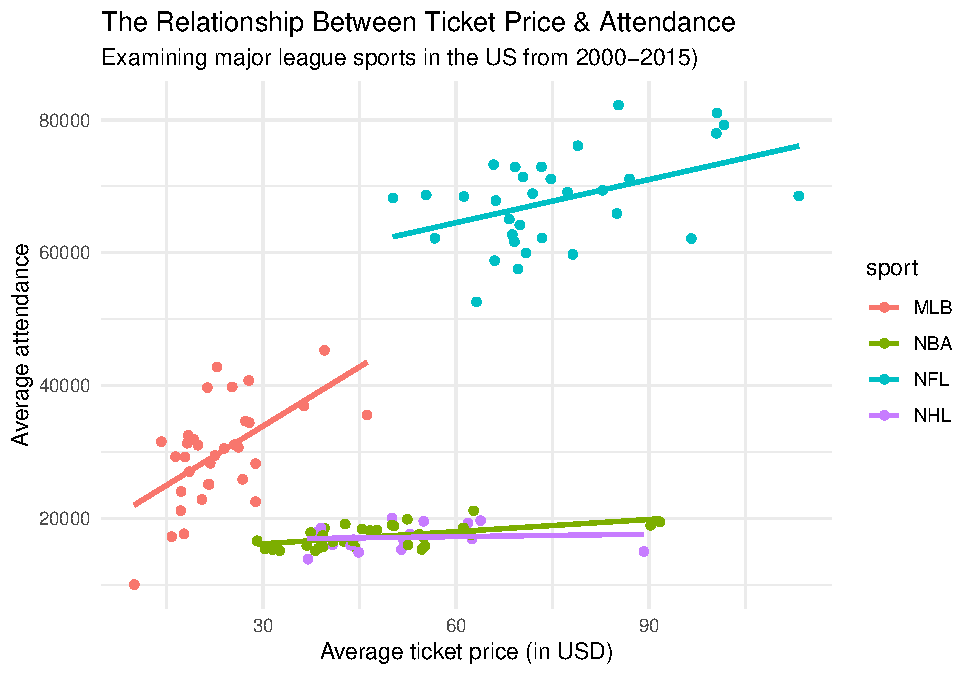
\includegraphics{Final_Project_files/figure-latex/plots-1.pdf}

\begin{Shaded}
\begin{Highlighting}[]
\NormalTok{sports_rev }\OperatorTok
\StringTok{  }\KeywordTok{ggplot}\NormalTok{(}\KeywordTok{aes}\NormalTok{(avg_ticket_price, avg_attendance, }\DataTypeTok{color =}\NormalTok{ sport)) }\OperatorTok{+}\StringTok{   }\KeywordTok{facet_wrap}\NormalTok{(}\OperatorTok{~}\NormalTok{sport) }\OperatorTok{+}
\StringTok{  }\KeywordTok{geom_point}\NormalTok{() }\OperatorTok{+}
\StringTok{  }\KeywordTok{geom_smooth}\NormalTok{(}\DataTypeTok{method =}\NormalTok{ lm, }\DataTypeTok{se =} \OtherTok{FALSE}\NormalTok{) }\OperatorTok{+}\StringTok{ }
\StringTok{  }\KeywordTok{labs}\NormalTok{(}\DataTypeTok{x =} \StringTok{"Average ticket price (in USD)"}\NormalTok{, }
       \DataTypeTok{y =} \StringTok{"Average attendance"}\NormalTok{, }
       \DataTypeTok{title =} \StringTok{"The Relationship Between Ticket Price & Attendance"}\NormalTok{,}
       \DataTypeTok{subtitle =} \StringTok{"Examining major league sports in the US from 2000-2015"}\NormalTok{) }\OperatorTok{+}
\StringTok{  }\KeywordTok{theme_minimal}\NormalTok{() }
\end{Highlighting}
\end{Shaded}

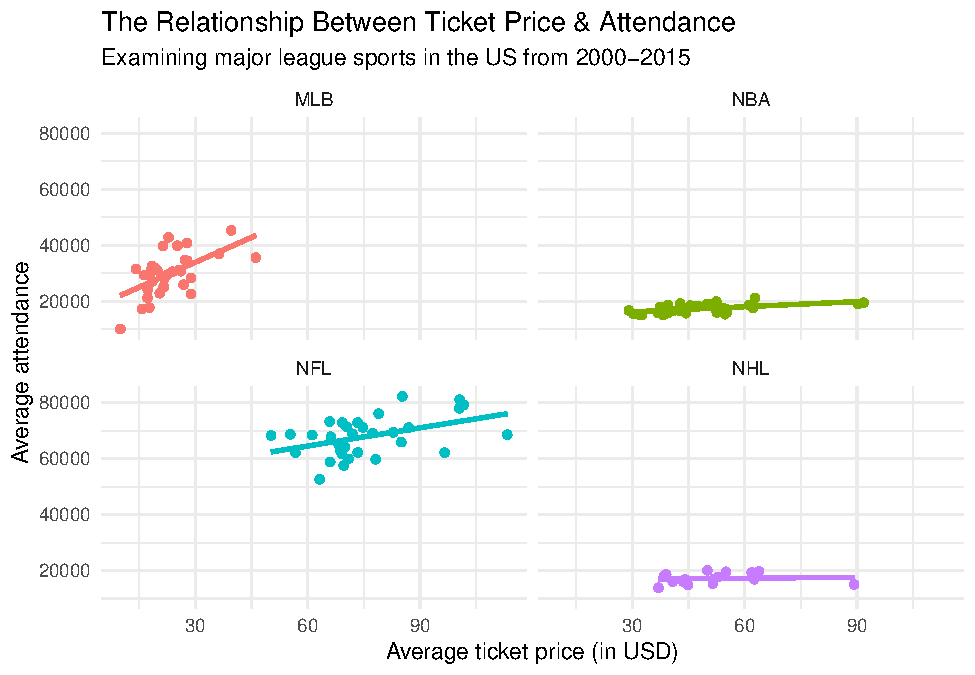
\includegraphics{Final_Project_files/figure-latex/plots-2.pdf}

\begin{Shaded}
\begin{Highlighting}[]
\NormalTok{sports_rev }\OperatorTok
\StringTok{  }\KeywordTok{ggplot}\NormalTok{(}\KeywordTok{aes}\NormalTok{(avg_homewinspct, avg_attendance, }\DataTypeTok{color =}\NormalTok{ sport)) }\OperatorTok{+}
\StringTok{  }\KeywordTok{geom_point}\NormalTok{() }\OperatorTok{+}
\StringTok{  }\KeywordTok{geom_smooth}\NormalTok{(}\DataTypeTok{method =}\NormalTok{ lm, }\DataTypeTok{se =} \OtherTok{FALSE}\NormalTok{) }\OperatorTok{+}\StringTok{ }
\StringTok{   }\KeywordTok{labs}\NormalTok{(}\DataTypeTok{x =} \StringTok{"Average Percent of Wins at Home Stadium"}\NormalTok{, }
       \DataTypeTok{y =} \StringTok{"Average attendance"}\NormalTok{, }
       \DataTypeTok{title =} \StringTok{"The Relationship Home Wins and Attendance"}\NormalTok{,}
       \DataTypeTok{subtitle =} \StringTok{"Examining major league sports in the US from 2000-2015"}\NormalTok{) }\OperatorTok{+}
\StringTok{  }\KeywordTok{theme_minimal}\NormalTok{()}
\end{Highlighting}
\end{Shaded}

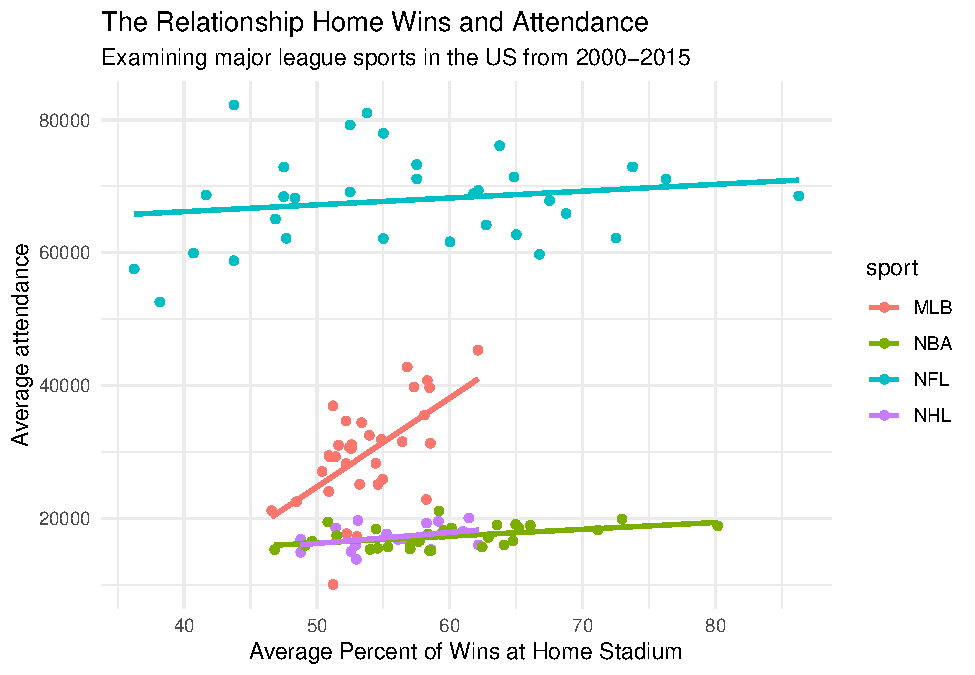
\includegraphics{Final_Project_files/figure-latex/plots-3.pdf}

\begin{Shaded}
\begin{Highlighting}[]
\NormalTok{sports_rev }\OperatorTok
\StringTok{  }\KeywordTok{ggplot}\NormalTok{(}\KeywordTok{aes}\NormalTok{(avg_homewinspct, avg_attendance, }\DataTypeTok{color =}\NormalTok{ sport)) }\OperatorTok{+}
\StringTok{  }\KeywordTok{facet_wrap}\NormalTok{(}\OperatorTok{~}\NormalTok{sport)}\OperatorTok{+}
\StringTok{  }\KeywordTok{geom_point}\NormalTok{() }\OperatorTok{+}
\StringTok{  }\KeywordTok{geom_smooth}\NormalTok{(}\DataTypeTok{method =}\NormalTok{ lm, }\DataTypeTok{se =} \OtherTok{FALSE}\NormalTok{) }\OperatorTok{+}\StringTok{ }
\StringTok{   }\KeywordTok{labs}\NormalTok{(}\DataTypeTok{x =} \StringTok{"Average Percent of Wins at Home Stadium"}\NormalTok{, }
       \DataTypeTok{y =} \StringTok{"Average attendance"}\NormalTok{, }
       \DataTypeTok{title =} \StringTok{"The Relationship Home Wins and Attendance"}\NormalTok{,}
       \DataTypeTok{subtitle =} \StringTok{"Examining major league sports in the US from 2000-2015"}\NormalTok{) }\OperatorTok{+}
\StringTok{  }\KeywordTok{theme_minimal}\NormalTok{()}
\end{Highlighting}
\end{Shaded}

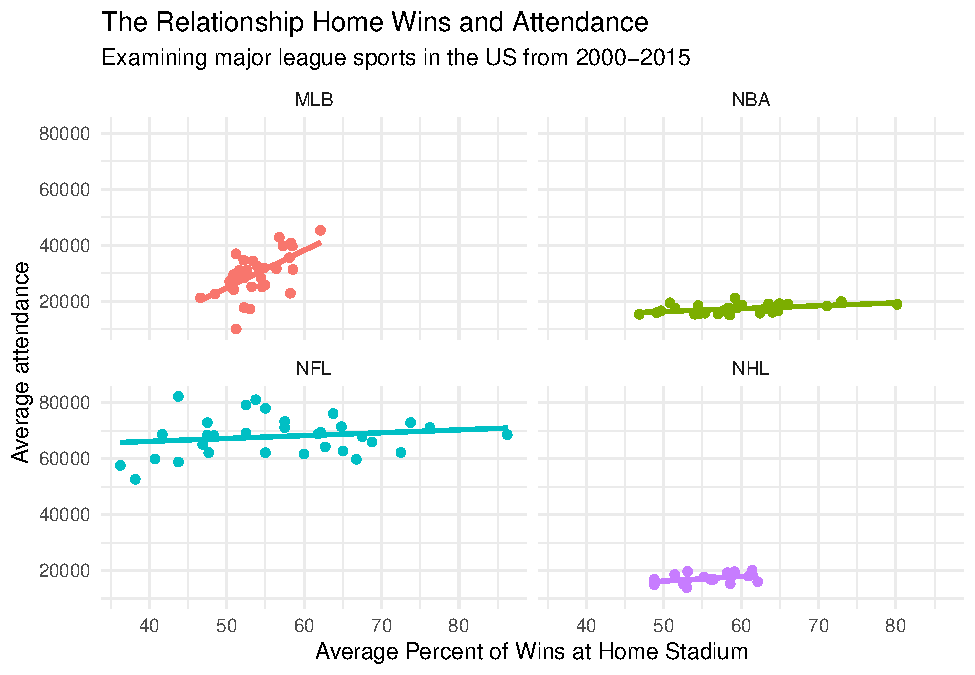
\includegraphics{Final_Project_files/figure-latex/plots-4.pdf}

\begin{Shaded}
\begin{Highlighting}[]
\NormalTok{sports_crisis <-}\StringTok{ }\NormalTok{sports }\OperatorTok
\StringTok{  }\KeywordTok{group_by}\NormalTok{(year, sport) }\OperatorTok
\StringTok{  }\KeywordTok{summarize}\NormalTok{(}\DataTypeTok{avg_ticket_price =} \KeywordTok{mean}\NormalTok{(ticket_price), }
            \DataTypeTok{avg_attendance =} \KeywordTok{mean}\NormalTok{(attend_avg)) }

\NormalTok{sports_crisis }\OperatorTok
\StringTok{  }\KeywordTok{filter}\NormalTok{(year }\OperatorTok{>=}\StringTok{ }\DecValTok{2005}\NormalTok{, year }\OperatorTok{<=}\StringTok{ }\DecValTok{2013}\NormalTok{) }\OperatorTok
\StringTok{  }\KeywordTok{ggplot}\NormalTok{(}\KeywordTok{aes}\NormalTok{(year, avg_ticket_price, }\DataTypeTok{color =}\NormalTok{ sport)) }\OperatorTok{+}
\StringTok{  }\KeywordTok{geom_line}\NormalTok{() }\OperatorTok{+}
\StringTok{  }\KeywordTok{labs}\NormalTok{ (}\DataTypeTok{x =} \StringTok{"Year"}\NormalTok{, }
        \DataTypeTok{y =} \StringTok{"Average Ticket Price (in USD)"}\NormalTok{, }
        \DataTypeTok{title =} \StringTok{"Major League Sport Ticket Prices During a Financial Crisis"}\NormalTok{,}
        \DataTypeTok{subtitle =} \StringTok{"Prices in USD from 2005 to 2013"}\NormalTok{) }\OperatorTok{+}
\StringTok{  }\KeywordTok{theme_minimal}\NormalTok{()}
\end{Highlighting}
\end{Shaded}

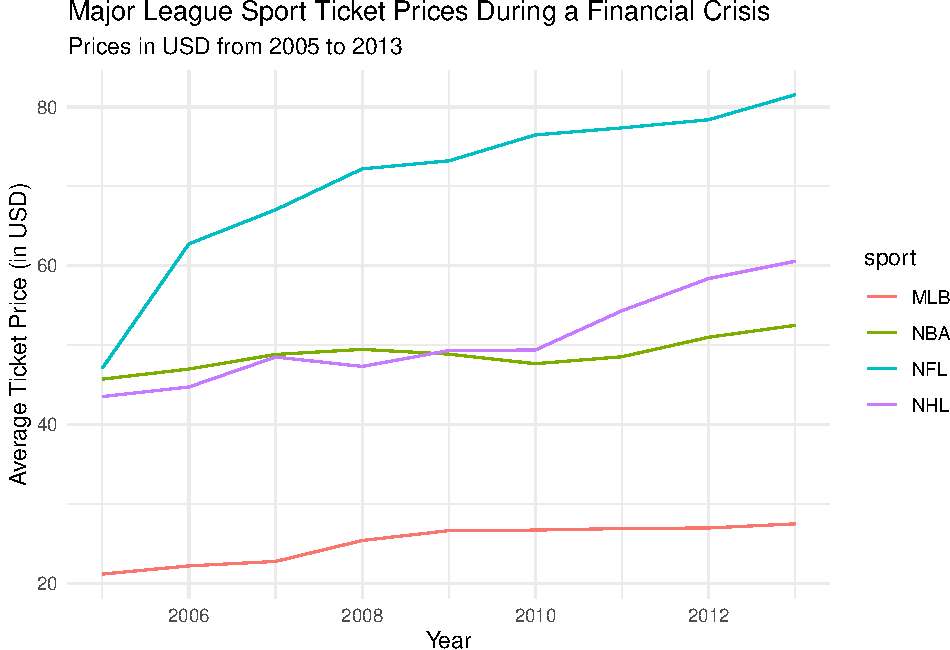
\includegraphics{Final_Project_files/figure-latex/sports_crisis-1.pdf}

\begin{Shaded}
\begin{Highlighting}[]
\NormalTok{sports_crisis }\OperatorTok
\StringTok{  }\KeywordTok{filter}\NormalTok{(year }\OperatorTok{>=}\StringTok{ }\DecValTok{2005}\NormalTok{, year }\OperatorTok{<=}\StringTok{ }\DecValTok{2013}\NormalTok{) }\OperatorTok
\StringTok{  }\KeywordTok{ggplot}\NormalTok{(}\KeywordTok{aes}\NormalTok{(year, avg_attendance, }\DataTypeTok{color =}\NormalTok{ sport)) }\OperatorTok{+}
\StringTok{  }\KeywordTok{facet_wrap}\NormalTok{(}\OperatorTok{~}\NormalTok{sport) }\OperatorTok{+}
\StringTok{  }\KeywordTok{geom_line}\NormalTok{() }\OperatorTok{+}
\StringTok{   }\KeywordTok{labs}\NormalTok{ (}\DataTypeTok{x =} \StringTok{"Year"}\NormalTok{, }
        \DataTypeTok{y =} \StringTok{"Average Attendence"}\NormalTok{, }
        \DataTypeTok{title =} \StringTok{"Major League Sport Attendence During a Financial Crisis"}\NormalTok{,}
        \DataTypeTok{subtitle =} \StringTok{"Prices in USD from 2005 to 2013"}\NormalTok{) }\OperatorTok{+}
\StringTok{  }\KeywordTok{theme_minimal}\NormalTok{()}
\end{Highlighting}
\end{Shaded}

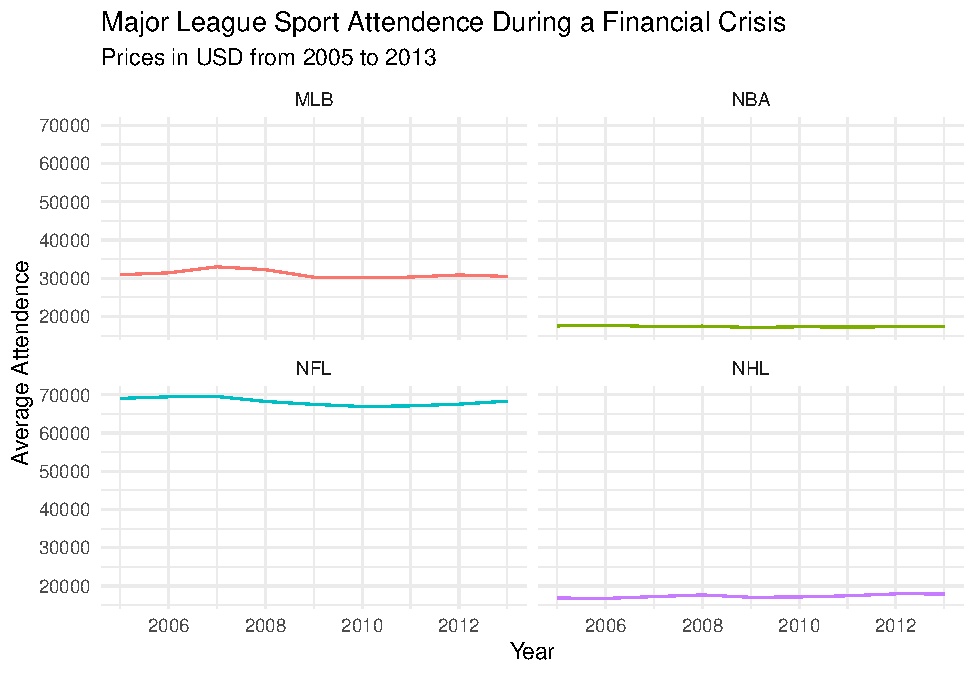
\includegraphics{Final_Project_files/figure-latex/sports_crisis-2.pdf}

\begin{Shaded}
\begin{Highlighting}[]
\NormalTok{fit =}\StringTok{ }\NormalTok{sports }\OperatorTok
\StringTok{  }\KeywordTok{group_by}\NormalTok{(sport) }\OperatorTok
\StringTok{  }\KeywordTok{do}\NormalTok{(}\DataTypeTok{model =} \KeywordTok{lm}\NormalTok{(attend_avg }\OperatorTok{~}\StringTok{ }\NormalTok{ticket_price }\OperatorTok{+}\StringTok{ }\NormalTok{home_wins_pct, }\DataTypeTok{data =}\NormalTok{ .))}
  
\NormalTok{sports_rev }\OperatorTok
\StringTok{  }\KeywordTok{filter}\NormalTok{(sport }\OperatorTok{==}\StringTok{ "MLB"}\NormalTok{) }\OperatorTok
\StringTok{  }\KeywordTok{ggplot}\NormalTok{(}\KeywordTok{aes}\NormalTok{(avg_homewinspct, avg_attendance)) }\OperatorTok{+}
\StringTok{  }\KeywordTok{geom_point}\NormalTok{() }\OperatorTok{+}
\StringTok{  }\KeywordTok{geom_smooth}\NormalTok{(}\DataTypeTok{se =} \OtherTok{FALSE}\NormalTok{)}\OperatorTok{+}
\StringTok{  }\KeywordTok{labs}\NormalTok{(}\DataTypeTok{x =} \StringTok{"Average percent of home wins"}\NormalTok{,}
       \DataTypeTok{y =} \StringTok{"Average attendance"}\NormalTok{, }
       \DataTypeTok{title =} \StringTok{"The Relationship Between Average Percent of Home Wins and Attendance"}\NormalTok{,}
       \DataTypeTok{subtitle =} \StringTok{"MLB statistics from 2000-2015"}\NormalTok{)}\OperatorTok{+}
\StringTok{  }\KeywordTok{theme_minimal}\NormalTok{()}
\end{Highlighting}
\end{Shaded}

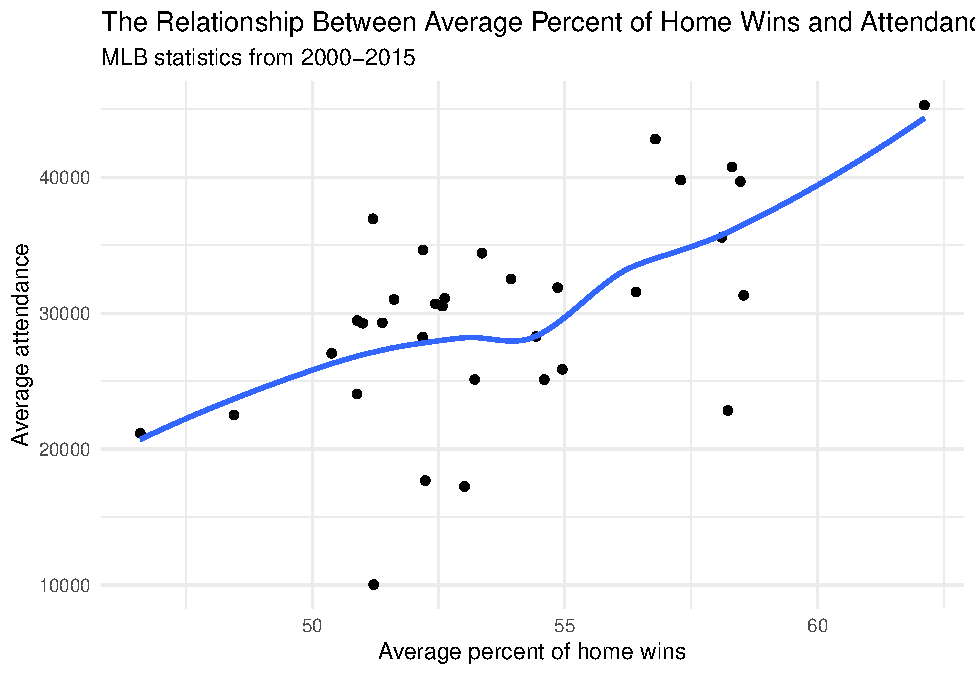
\includegraphics{Final_Project_files/figure-latex/sports_crisis-3.pdf}

\hypertarget{average-home-attendance-average-home-ticket-price-and-average-home-win-pct-by-sports-2000-2015}{%
\subsection{Average Home Attendance, Average Home Ticket Price and Average Home Win pct by Sports (2000-2015)}\label{average-home-attendance-average-home-ticket-price-and-average-home-win-pct-by-sports-2000-2015}}

\begin{Shaded}
\begin{Highlighting}[]
\NormalTok{sports }\OperatorTok
\StringTok{  }\KeywordTok{group_by}\NormalTok{(sport) }\OperatorTok
\StringTok{  }\KeywordTok{summarize}\NormalTok{(}\DataTypeTok{avg_attendance =} \KeywordTok{mean}\NormalTok{(attend_avg),}
            \DataTypeTok{avg_ticket_price =} \KeywordTok{mean}\NormalTok{(ticket_price), }
            \DataTypeTok{avg_homewinspct =} \KeywordTok{mean}\NormalTok{(home_wins_pct)) }\OperatorTok
\StringTok{  }\KeywordTok{kable}\NormalTok{(}\DataTypeTok{digits =} \DecValTok{2}\NormalTok{,}
        \DataTypeTok{col.names =} \KeywordTok{c}\NormalTok{(}\StringTok{"sport"}\NormalTok{, }\StringTok{"attendance_mean"}\NormalTok{, }\StringTok{"ticketprice_mean"}\NormalTok{, }\StringTok{"homewinpct_mean"}\NormalTok{), }\DataTypeTok{format =} \StringTok{"latex"}\NormalTok{)}
\end{Highlighting}
\end{Shaded}

\begin{tabular}{l|r|r|r}
\hline
sport & attendance\_mean & ticketprice\_mean & homewinpct\_mean\\
\hline
MLB & 30420.90 & 23.51 & 53.88\\
\hline
NBA & 17335.68 & 49.04 & 59.70\\
\hline
NFL & 68039.56 & 75.29 & 56.86\\
\hline
NHL & 17342.74 & 51.76 & 55.94\\
\hline
\end{tabular}

\begin{Shaded}
\begin{Highlighting}[]
\NormalTok{sports_crisis_before <-}\StringTok{ }\NormalTok{sports }\OperatorTok
\StringTok{  }\KeywordTok{filter}\NormalTok{(sport }\OperatorTok{==}\StringTok{ "MLB"}\NormalTok{, year }\OperatorTok{>=}\StringTok{ }\DecValTok{2007}\NormalTok{, year }\OperatorTok{<=}\StringTok{ }\DecValTok{2009}\NormalTok{)}

\NormalTok{sports_crisis_after <-}\StringTok{ }\NormalTok{sports }\OperatorTok
\StringTok{  }\KeywordTok{filter}\NormalTok{(sport }\OperatorTok{==}\StringTok{ "MLB"}\NormalTok{, year }\OperatorTok{>=}\StringTok{ }\DecValTok{2010}\NormalTok{, year }\OperatorTok{<=}\StringTok{ }\DecValTok{2012}\NormalTok{)}
  
\NormalTok{attendance_before <-}\StringTok{ }\KeywordTok{mean}\NormalTok{(sports_crisis_before}\OperatorTok{$}\NormalTok{attend_avg, }\DataTypeTok{na.rm =} \OtherTok{TRUE}\NormalTok{)}
\NormalTok{price_before <-}\StringTok{ }\KeywordTok{mean}\NormalTok{(sports_crisis_before}\OperatorTok{$}\NormalTok{ticket_price, }\DataTypeTok{na.rm =} \OtherTok{TRUE}\NormalTok{)}
\NormalTok{attendance_after <-}\StringTok{ }\KeywordTok{mean}\NormalTok{(sports_crisis_after}\OperatorTok{$}\NormalTok{attend_avg, }\DataTypeTok{na.rm =} \OtherTok{TRUE}\NormalTok{)}
\NormalTok{price_after <-}\StringTok{ }\KeywordTok{mean}\NormalTok{(sports_crisis_after}\OperatorTok{$}\NormalTok{ticket_price, }\DataTypeTok{na.rm =} \OtherTok{TRUE}\NormalTok{)}
\end{Highlighting}
\end{Shaded}

\hypertarget{average-home-game-revenue-before-and-after-economic-recession}{%
\subsection{Average Home Game Revenue before and after economic recession}\label{average-home-game-revenue-before-and-after-economic-recession}}

Average revenue per homegame of MLB spanning from 2007 and 2009 is \$794,445.22 while the one for 3 years after \textbf{financial crisis} is \$818,114.18. Major League Baseball seems that it was not affected by depression in terms of \emph{revenue} and it actually made more than before the crisis.

\begin{Shaded}
\begin{Highlighting}[]
\NormalTok{sports_pivot <-}\StringTok{ }\NormalTok{sports }\OperatorTok
\StringTok{  }\KeywordTok{pivot_longer}\NormalTok{(home_wins, }\DataTypeTok{names_to =} \KeywordTok{c}\NormalTok{(}\StringTok{"home"}\NormalTok{, }\StringTok{"wins"}\NormalTok{), }\DataTypeTok{names_sep =} \StringTok{"_"}\NormalTok{, }\DataTypeTok{values_to =} \StringTok{"victory"}\NormalTok{) }\OperatorTok
\StringTok{  }\KeywordTok{pivot_wider}\NormalTok{(}\DataTypeTok{names_from =}\NormalTok{ wins, }\DataTypeTok{values_from =}\NormalTok{ victory) }\OperatorTok
\StringTok{  }\KeywordTok{select}\NormalTok{(}\OperatorTok{-}\KeywordTok{c}\NormalTok{(}\DecValTok{9}\NormalTok{)) }\OperatorTok
\StringTok{  }\KeywordTok{rename}\NormalTok{(}\DataTypeTok{home_wins =}\NormalTok{ wins)}
\end{Highlighting}
\end{Shaded}

\hypertarget{methods}{%
\section{Methods}\label{methods}}

The sports dataset comes from marketing professor Conor Henderson. It covers four major league sports (NBA, MLB, NFL, NHL) as well as NCAA college football. For each sport, the data spans from 2000 through 2015 and is currently in the process of being updated through present. The data was originally compiled from a number of reputable sports-focused sources including Rodney Fort's Sports League Database as well as ESPN.
In the final dataset that combines all the sports we have 1398 observations across 15 years and 10 different variables. The 10 variables we selected were: sport, team, year, stadium capacity, total attendance, average attendance, number of games, ticket price (in USD), and the number of home wins.

\hypertarget{data-analysis}{%
\subsection{Data analysis}\label{data-analysis}}

We used R (Version 3.6.1; R Core Team, 2019) and the R-packages \emph{dplyr} (Version 0.8.3; Wickham et al., 2019), \emph{forcats} (Version 0.4.0; Wickham, 2019a), \emph{ggplot2} (Version 3.2.1; Wickham, 2016), \emph{here} (Version 0.1; Müller, 2017), \emph{janitor} (Version 1.2.0; Firke, 2019), \emph{kableExtra} (Version 1.1.0; Zhu, 2019), \emph{knitr} (Version 1.25; Xie, 2015), \emph{lme4} (Version 1.1.21; Bates, Mächler, Bolker, \& Walker, 2015), \emph{Matrix} (Version 1.2.17; Bates \& Maechler, 2019), \emph{papaja} (Version 0.1.0.9842; Aust \& Barth, 2018), \emph{purrr} (Version 0.3.2; Henry \& Wickham, 2019), \emph{readr} (Version 1.3.1; Wickham, Hester, \& Francois, 2018), \emph{rio} (Version 0.5.16; Chan, Chan, Leeper, \& Becker, 2018), \emph{stringr} (Version 1.4.0; Wickham, 2019b), \emph{tibble} (Version 2.1.3; Müller \& Wickham, 2019), \emph{tidyr} (Version 1.0.0; Wickham \& Henry, 2019), and \emph{tidyverse} (Version 1.2.1; Wickham, 2017) for all our analyses.

\hypertarget{results}{%
\section{Results}\label{results}}

In all four leagues, it turns out that average ticket price and average home win rate have a positive relationship with average home attendance even though NFL fans seem to be not as sensitive to win as other three leagues' fans are. In addition, the 2008 financial crisis did not result in crisis in the US professional sports leagues. While some of the leagues experienced slight decrease in home attendance, all four leagues got through economic downturn as if there was nothing happened. Actually, their home game average revenue went up after financial crisis. We assume this counterintuitive outcome is attributed to the facts that sports were kind of immuned to the crisis for some reason or even during recession people are willing to spend money for watching games.

\hypertarget{discussion}{%
\section{Discussion}\label{discussion}}

Sports continue to play an important role in the United States. In an time when individuals are becoming increasingly isolated {[}Chalmers2012differences;Shachar2011brands{]}, sports games provide a form of entertainment that can be bring people together, whether that be through watching the game at the sadium or field or on television. While the motivation to watch sports differs for individuals, the widespread appeal of watching teams compete provides a context for marketers to understand sponshorship, group marketing strategies, and targeted advertising.
The current exploratory study provides inital insight into how major league attendance varries over time both in regard to attedance as well as ticket prices. Through the analysis, it is clear that each of the major league sports operates very differently from eachother inregard to the variables of interest isolated for the purposes of this research.
As this dataset it used going forward, it will be important to identify more clearly the differences between each of the sports to understand if they can indeed be collapsed into an overarching category of \enquote{major league sports attendance} across all four major league sports (MLB, NBA, NFL, NHL). Another aspect that was not taken into account in the current research is team-specific factors including how long the team has been in a city as well as how many time a team has moved.

\newpage

\hypertarget{references}{%
\section{References}\label{references}}

\begin{Shaded}
\begin{Highlighting}[]
\KeywordTok{r_refs}\NormalTok{(}\DataTypeTok{file =} \StringTok{"r-references.bib"}\NormalTok{)}
\end{Highlighting}
\end{Shaded}

\begingroup
\setlength{\parindent}{-0.5in}
\setlength{\leftskip}{0.5in}

\hypertarget{refs}{}
\leavevmode\hypertarget{ref-R-papaja}{}%
Aust, F., \& Barth, M. (2018). \emph{papaja: Create APA manuscripts with R Markdown}. Retrieved from \url{https://github.com/crsh/papaja}

\leavevmode\hypertarget{ref-R-Matrix}{}%
Bates, D., \& Maechler, M. (2019). \emph{Matrix: Sparse and dense matrix classes and methods}. Retrieved from \url{https://CRAN.R-project.org/package=Matrix}

\leavevmode\hypertarget{ref-R-lme4}{}%
Bates, D., Mächler, M., Bolker, B., \& Walker, S. (2015). Fitting linear mixed-effects models using lme4. \emph{Journal of Statistical Software}, \emph{67}(1), 1--48. doi:\href{https://doi.org/10.18637/jss.v067.i01}{10.18637/jss.v067.i01}

\leavevmode\hypertarget{ref-R-rio}{}%
Chan, C.-h., Chan, G. C., Leeper, T. J., \& Becker, J. (2018). \emph{Rio: A swiss-army knife for data file i/o}.

\leavevmode\hypertarget{ref-coates_humphreys_2007}{}%
Coates, D., \& Humphreys, B. R. (2007). Ticket prices, concessions and attendance at professional sporting events. \emph{International Journal of Sport Finance}, \emph{2}(3), 161.

\leavevmode\hypertarget{ref-R-janitor}{}%
Firke, S. (2019). \emph{Janitor: Simple tools for examining and cleaning dirty data}. Retrieved from \url{https://CRAN.R-project.org/package=janitor}

\leavevmode\hypertarget{ref-R-purrr}{}%
Henry, L., \& Wickham, H. (2019). \emph{Purrr: Functional programming tools}. Retrieved from \url{https://CRAN.R-project.org/package=purrr}

\leavevmode\hypertarget{ref-humphreys_2010}{}%
Humphreys, B. R. (2010). The impact of the global financial crisis on sport in north america. In \emph{Optimal strategies in sports economics and management} (pp. 39--57). Springer.

\leavevmode\hypertarget{ref-R-here}{}%
Müller, K. (2017). \emph{Here: A simpler way to find your files}. Retrieved from \url{https://CRAN.R-project.org/package=here}

\leavevmode\hypertarget{ref-R-tibble}{}%
Müller, K., \& Wickham, H. (2019). \emph{Tibble: Simple data frames}. Retrieved from \url{https://CRAN.R-project.org/package=tibble}

\leavevmode\hypertarget{ref-R-base}{}%
R Core Team. (2019). \emph{R: A language and environment for statistical computing}. Vienna, Austria: R Foundation for Statistical Computing. Retrieved from \url{https://www.R-project.org/}

\leavevmode\hypertarget{ref-R-ggplot2}{}%
Wickham, H. (2016). \emph{Ggplot2: Elegant graphics for data analysis}. Springer-Verlag New York. Retrieved from \url{https://ggplot2.tidyverse.org}

\leavevmode\hypertarget{ref-R-tidyverse}{}%
Wickham, H. (2017). \emph{Tidyverse: Easily install and load the 'tidyverse'}. Retrieved from \url{https://CRAN.R-project.org/package=tidyverse}

\leavevmode\hypertarget{ref-R-forcats}{}%
Wickham, H. (2019a). \emph{Forcats: Tools for working with categorical variables (factors)}. Retrieved from \url{https://CRAN.R-project.org/package=forcats}

\leavevmode\hypertarget{ref-R-stringr}{}%
Wickham, H. (2019b). \emph{Stringr: Simple, consistent wrappers for common string operations}. Retrieved from \url{https://CRAN.R-project.org/package=stringr}

\leavevmode\hypertarget{ref-R-dplyr}{}%
Wickham, H., François, R., Henry, L., \& Müller, K. (2019). \emph{Dplyr: A grammar of data manipulation}. Retrieved from \url{https://CRAN.R-project.org/package=dplyr}

\leavevmode\hypertarget{ref-R-tidyr}{}%
Wickham, H., \& Henry, L. (2019). \emph{Tidyr: Tidy messy data}. Retrieved from \url{https://CRAN.R-project.org/package=tidyr}

\leavevmode\hypertarget{ref-R-readr}{}%
Wickham, H., Hester, J., \& Francois, R. (2018). \emph{Readr: Read rectangular text data}. Retrieved from \url{https://CRAN.R-project.org/package=readr}

\leavevmode\hypertarget{ref-R-knitr}{}%
Xie, Y. (2015). \emph{Dynamic documents with R and knitr} (2nd ed.). Boca Raton, Florida: Chapman; Hall/CRC. Retrieved from \url{https://yihui.name/knitr/}

\leavevmode\hypertarget{ref-R-kableExtra}{}%
Zhu, H. (2019). \emph{KableExtra: Construct complex table with 'kable' and pipe syntax}. Retrieved from \url{https://CRAN.R-project.org/package=kableExtra}

\endgroup


\end{document}
